\section{Tensões induzidas em circuitos paralelos}

Em operação normal as tensões são impostas pelos geradores, pois a sua conexão com a linha é feita por uma impedância menor que as de acoplamento. Quando o circuito sai de operação, a impedância de conexão com o solo passa a ser tão grande quanto as de acoplamento, permitindo que as tensões sejam determinadas por essas impedâncias em um acoplamento capacitivo e indutivo.

Durante a conexão entre circuitos será considerado o modelo apenas por acoplamento capacitivo devido a sua maior influência. O efeito indutivo pode ser utilizado para refinamento. O problema é formulado a partir da matriz admitância de capacitâncias considerando uma linha transposta.

Assim, em termos de circuito duplo a matriz de admitâncias será representada por uma composição de submatrizes simétricas e balanceadas na forma matricial compacta:

\begin{equation} \label{slide:3:1}
    Y_{abc} \, = \,\begin{bmatrix} Y_{11(abc)} & Y_{12(abc)} \\ Y_{12(abc)} & Y_{22(abc)}   \end{bmatrix}
\end{equation}

Onde as matrizes $Y_{11(abc)}$ e  $Y_{22(abc)}$ representam as matrizes com as respectivas capacitâncias próprias (diagonal) e mútuas entre as fases dentro do circuito em questão. Enquanto que as matrizes $Y_{12(abc)}=Y_{21(abc)}$ se referem às capacitâncias mútuas entre as fases do circuito um para as fases do circuito 2.

A representação em componentes simétricas pode ser obtida ao aplicar a matriz de transformação para a forma compacta:

\begin{equation} \label{slide:3:2}
    Y_{012} \, = \, \begin{bmatrix} T^{-1} &   \\  & T^{-1}  \end{bmatrix}  \times \begin{bmatrix} Y_{11(abc)} & Y_{12(abc)} \\ Y_{12(abc)} & Y_{22(abc)}   \end{bmatrix} \times \begin{bmatrix} T &   \\  & T  \end{bmatrix} 
\end{equation}

Aplicando essa matriz nas tensões de sequência positiva de ambos os circuitos ($[v_{1(012)} v_{2(012)}]$), obtém-se o vetor das correntes ($[i_{1(012)} i_{2(012)}]$). Esses vetores são uma composição de dois vetores trifásicos para a grandeza em questão de cada circuito.

\begin{figure}[H]
\begin{center}
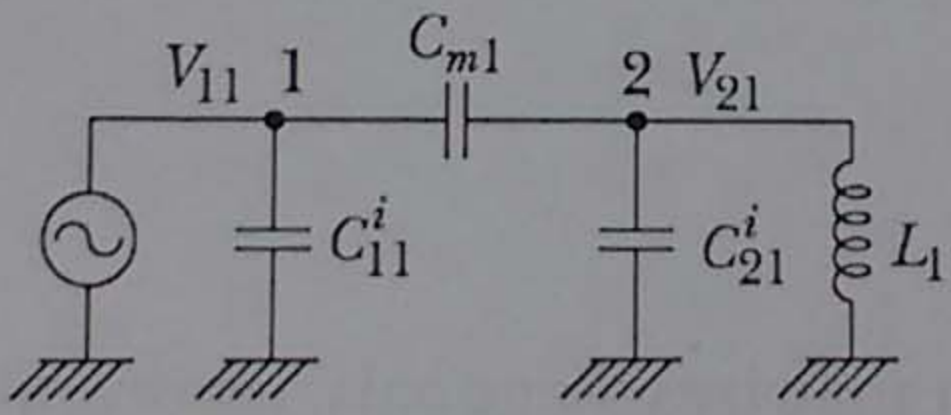
\includegraphics[width=8cm]{images/seq_pos_reator.png}
\caption{Circuito transposto de sequência positiva com reator. Fonte: Júnior, 2003.}
\label{slide3:seq_pos_reat} 
\end{center}
\end{figure}

Após a transposição, ainda consta-se a presença de capacitâncias mútuas entre sequências no circuito da figura \ref{slide3:seq_pos_reat}. Implicando que ao alimentar o circuito 1 com uma tensão de sequência X, uma tensão induzida referente a sequência X será gerada no circuito 2.

Pelo divisor de tensão no circuito transposto desconsiderando a reatância, fica claro que a tensão $V_{21}$ será menor que a tensão $V_{11}$. O emprego de reatores no fim da linha permitem que a situação de tensão possa se reverter, pois eles alteram as relações de impedância do divisor de tensão.

Realizando a análise com a presença de um reator aterrado com um reator de neutro, obtendo o circuito de sequência positiva da figura \ref{slide3:seq_pos_reat}. Em termos das matrizes, a mudança é obtida na matriz $Y_{22(012)}$, que agora, em sua diagonal principal possui seus elementos somados com as reatâncias de componentes de sequência. A consequência direta nas correntes será:

\begin{equation} \label{slide:3:3}
    \begin{bmatrix} i_{1(012)}  \\ i_{2(012)} + i_{r(012)}  \end{bmatrix} \, = \,\begin{bmatrix} Y_{11(012)} & Y_{12(012)} \\ Y_{12(012)} & Y_{22(012)}^{'}  \end{bmatrix} \times \begin{bmatrix} v_{1(012)}  \\ v_{2(012)}  \end{bmatrix}
\end{equation}

Para evidenciar as condições ressonantes, faz-se o equacionamento das correntes por meio da lei de Kirchoff para o circuito 2 na figura \ref{slide3:seq_pos_reat}:

\begin{equation} \label{slide:3:4}
    i_{2(012)} + i_{r(012)} = 0
\end{equation}

Reaplicando a condição de ressonância expressa em \ref{slide:3:4} de volta na equação matricial em \ref{slide:3:3}, obtém-se a seguinte relação entre as tensões dos circuitos:

\begin{center} 
    $v_{2(012)} = -Y_{22(012)}^{-1} Y_{21(012)} v_{1(012)}$
\end{center}

A expressão pode ser resumida em termos das admitâncias da matriz correspondente e em termos do circuito de sequência positiva, assim permitindo obter:

\begin{center}
    $V_{21} = -\frac{y_{m1}}{y_{21}+y_{r1}}V_{11}$
\end{center}

A condição ressonante é tal que: $y_{21}=-y_{r1}$. Com $y_{21} = j\omega C_{21}$ e $-y_{r1} = j/\omega L_1$. O termo $C_{21}$ é a soma de todas as capacitâncias no nó 2 da rede de sequência positiva: $C_{21} = C_{m1} + C_{21}^{i}$. Assim a frequência de ressonância da rede será:

\begin{equation} \label{slide:3:5}
    \omega = \frac{1}{\sqrt{(C_{m1} + C_{21}^{i})L_1}}
\end{equation}
    
Em geral a componente mútua da capacitância é muito baixa, podendo ser desconsiderada. As conclusões acima se refletem nos circuitos de componente negativa e zero.

